\documentclass[12pt]{article}

\usepackage{geometry}
\usepackage[T1]{fontenc}
\usepackage[utf8]{inputenc}
\usepackage[francais]{babel}

\usepackage{graphicx}
\usepackage{lmodern}
\usepackage{color}
\usepackage{listings}
\lstset{language=SQL, frame=shadowbox, rulesepcolor=\color{blue}}

\geometry{margin=2cm}


\begin{document}

\thispagestyle{empty}
\noindent
\includegraphics[width=0.25\textwidth]{enseirb-matmeca}

\vspace{\stretch{1}}

\begin{center}
	\Huge{\textbf{Rapport de projet SGBD :}}

	\Huge{\textbf{Bandes dessinées}}
\end{center}

\vspace{\stretch{2}}

\begin{tabular}{r@{:~}l}
	\textbf{Auteurs} & \textit{David Bitonneau, Ludovic Hofer, Benoît Ruelle}\\
 \textbf{Encadrants} & \textit{Mme. Allyx Fontaine, M. Sylvain Lombardy,
M. Mohamed Mosbah}\\
\end{tabular}

\vspace{\stretch{1}}

\begin{center}Deuxième année, filière informatique

	Date : \today
\end{center}

\newpage

\section{Introduction}

L'objectif du projet est de mettre en œuvre, sur un cas pratique, les notions
et les méthodes vues dans le module de SGBD. L'application effectuée ici est
liée à la gestion de bandes dessinées.

Dans ce rapport, la base de données est décrite de sa conception à son
utilisation, en passant par son implémentation. 

\section{Modélisation des données}

\subsection{Description du contexte de l'application}

\paragraph{}
L'application doit permettre la gestion de bandes dessinées à partir des
informations suivantes :

\begin{itemize}
	\item Chaque volume de bande dessinée est soit un album, soit une revue.
	\item Tout volume a un éditeur, et une année d’édition.
	\item Un album peut éventuellement appartenir à une collection, et dans ce cas, il
		peut avoir un numéro dans cette collection. Deux albums de la même collection
		ont forcément le même éditeur.
	\item Un volume a un titre, qui est soit le titre de l'album, soit celui de la
		revue ; dans le cas de la revue, elle a aussi un numéro.
	\item Un volume peut contenir plusieurs histoires.
	\item Chaque histoire a un titre et une année de (première) parution ; elle a un
		ou plusieurs auteurs, chacun de ces auteurs s’occupant du dessin ou du
		scénario (ou des deux).
	\item Une même histoire peut apparaître dans différents volumes ; on veut pouvoir
		annoter la présence d’une histoire dans un volume ("Première publication",
		"Pages 15 à 22", "Version longue", etc.).
	\item Une histoire peut appartenir à une série et dans ce cas elle peut avoir un
		numéro de série.
\end{itemize}

\paragraph{}
La lecture de ces informations fait ressortir les entités suivantes :
\begin{itemize}
	\item volume (regroupe les attributs communs des albums et des revues);
	\item album avec collection ;
	\item album sans collection ;
	\item revue ;
	\item éditeur ;
	\item collection ;
	\item histoire ;
	\item série d'histoires ;
	\item rôle d'un auteur ;
	\item auteur.
\end{itemize}

\paragraph{Les hypothèses suivantes sont effectuées :}
\begin{itemize}
	\item On considère qu'une revue est un ensemble de numéros de la revue et que l'éditeur d'une revue peut varier dans le temps.
	\item Plusieurs collections différentes peuvent avoir le même nom.
	\item On autorise que des histoires n'aient pas d'auteur renseigné ou que
		des volumes ou des collections ne soient pas associés à un éditeur
		présent dans la base. Inversement, des auteurs ou des éditeurs peuvent
		être présents dans la base sans être liés à une histoire, un volume ou
		une collection.
\end{itemize}


\section{Schéma conceptuel}

Le schéma conceptuel suivant montre les relations entre ces
différentes entités :

\noindent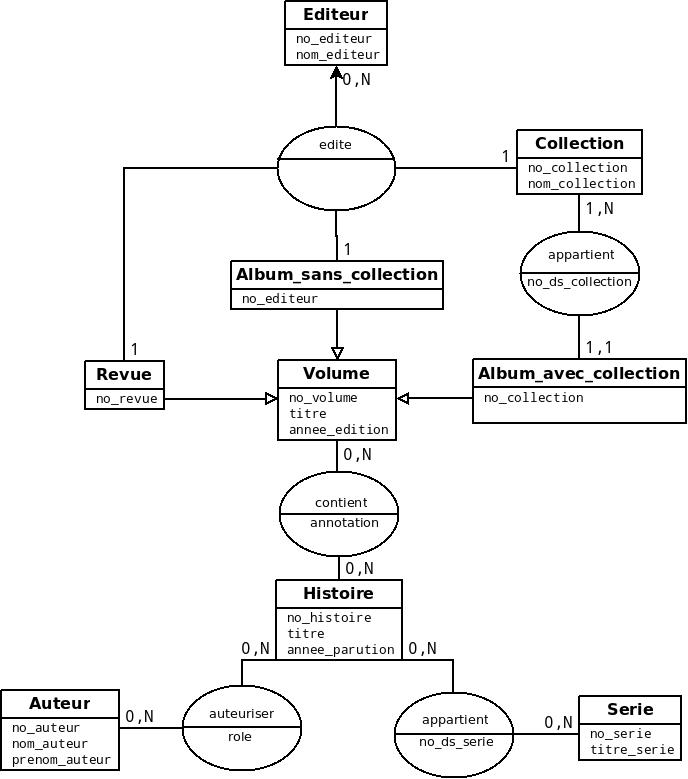
\includegraphics[width=\textwidth]{schema-conceptuel}


\section{Schéma relationnel}

\noindent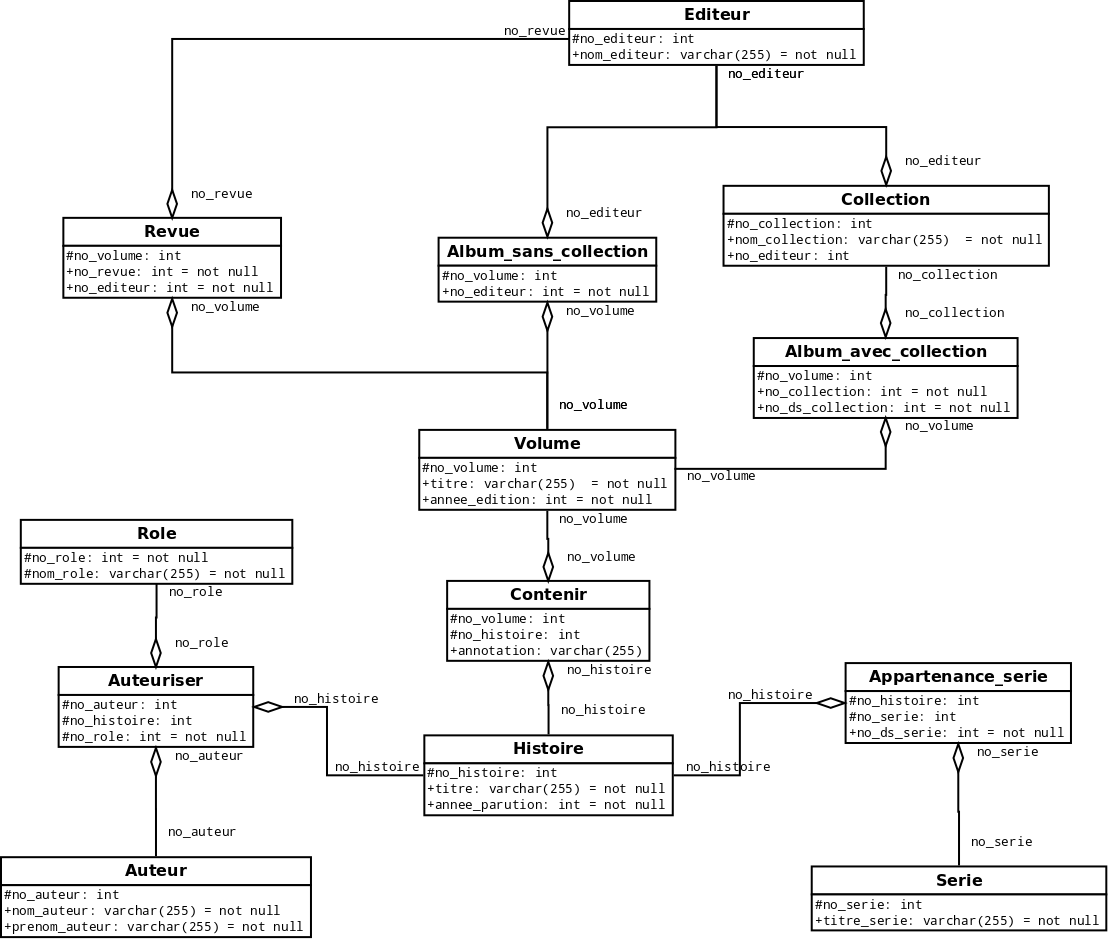
\includegraphics[width=\textwidth]{schema-relation}

\section{Implémentation}

La base a été implémentée en utilisant MySQL. Ce SGBD a été choisi pour sa
simplicité d'installation et de configuration.

\subsection{Contraintes d'intégrité, dépendances fonctionnelles}

Des contraintes d'intégrité sont réalisées au niveau de la plupart des clés
étrangères pour trois situations : 
\begin{itemize}
	\item Réaliser des suppressions en cascade d'entrées. C'est le cas par
		exemple de la suppression automatique de relations 'contenir'
		lorsqu'un album ou une histoire est supprimée ou de relations
		'auteuriser' dans le cas de la suppression d'auteurs ou d'histoires.
	\item Mettre des valeurs par défaut (null) dans les attributs concernant les
		éditeurs (album sans collection, collection, revue) lorsqu'un éditeur
		est supprimé.
	\item Bloquer la suppression d'une collection s'il y
		a encore des albums dans cette collection.
\end{itemize}

Pour alléger le code de l'interface et limiter la duplication, des vues ont été créées. Elles permettent
par exemple d'associer des histoires à leurs auteurs en une requête simple sur
laquelle il suffit d'appliquer une condition supplémentaire pour isoler un
auteur particulier. La même chose est faite pour associer des albums à leur
collection ou leur éditeur, des volumes à leurs histoires etc.

Si la base devait gérer un très grand nombre d'entrées, il serait possible
d'améliorer les performances de ces requêtes en les construisant directement
dans l'interface en s'assurant de manipuler des tables moins grosses en
faisant une sélection dès le début.


\section{Opérations possibles sur la base}

Différentes opérations peuvent être effectuées sur la base de données.
Ces opérations peuvent être classées en 3 différentes catégories :
\begin{itemize}
	\item les opérations de consultation ;
	\item l'extraction de statistiques ;
	\item les mises à jour de la base.
\end{itemize}

\paragraph{Consultation}

Ces opérations permettent de fournir des informations basiques concernant
diverses entités de la base de données à partir des informations qui y sont
stockées.
Les informations suivantes sont notamment fournies :
\begin{itemize}
	\item la bibliographie d’un auteur, soit par ordre chronologique, soit classé par séries, en tant que
		scénariste, dessinateur ou auteur complet, en indiquant ses co-auteurs et leurs rôles.
	\item la liste des auteurs collaborant à une revue durant une certaine période, avec le nombre de
		numéros auxquels ils ont participé.
	\item l'historique de la publication d’une histoire.
	\item les histoires différentes ayant le même titre.
\end{itemize}

L'implémentation des requêtes permettant d'obtenir ces informations a été effectué en deux phases :
\begin{itemize}
  \item Écriture de requête non paramétrées dans un fichier sql et test du résultat.
  \item Inclusion des requêtes dans des fonctions php, en utilisant des paramètres.
\end{itemize}

Cette démarche a permis de concevoir et d'affiner les requêtes dans un cas assez simple pour
ensuite pouvoir les intégrer de manière efficace à notre interface. Certaines requêtes étant
compliquées, elles ont été conçues étape après étape, en s'approchant peu à peu du résultat. Il est évident
que pour ce genre de procédure, il est plus simple d'affiner le résultat en exécutant un fichier sql qu'en
passant directement par du php.


\paragraph{Statistiques}
Les statistiques suivantes peuvent être prélevées grâce aux requêtes
implémentée :
\begin{itemize}
	\item le nombre d’histoires auxquelles un auteur a participé ;
	\item la série ayant le plus grand nombre d’auteurs ;
	\item les histoires classées selon le nombre de fois où elles apparaissent en album ;
	\item le nombre moyen d’auteurs participant à une revue pendant une période donnée.
\end{itemize}

Les méthodes utilisées pour le développement des requêtes de statistiques sont
les mêmes que celles utilisées pour les requêtes de consultation. La requête
permettant de classer les auteurs selon la décade durant laquelle ils ont créé
le plus d'histoires n'a pas été développée, notre compréhension du résultat
attendu n'étant pas des plus précises. Cependant, nous avons tout de même
testé la possibilité d'afficher le nombre d'histoires ayant été écrites pour
chaque décade, il ne nous serait donc pas particulièrement difficile
d'afficher la décade durant laquelle un auteur spécifique a créé le plus
d'histoires. En revanche, il nous semble bien plus complexe d'effectuer cette
opération pour tous les auteurs simultanément.

\paragraph{Mise à jour}
Il est possible d'appliquer les opérations de modification de la tables
suivantes :
\begin{itemize}
	\item Ajout, suppression, modification d’une histoire, d’un volume, d’un
		auteur, d'une série.
	\item Création de collections rendant par la suite possible la création
		d'albums avec collection.
	\item Association d'histoires à des séries et à des auteurs.
\end{itemize}

\subsection{Explication détaillée des requêtes}

\subsubsection*{La bibliographie d'un auteur par ordre chronologique}
\begin{lstlisting}
SELECT DISTINCT *
 FROM auteuriser ai, histoire h
 WHERE ai.no_auteur = 2
 AND ai.no_histoire = h.no_histoire;
\end{lstlisting}
Cette requête consiste simplement à conserver les différentes histoires pour
lesquels une entrée contient le numéro d'auteur approprié dans la table
auteuriser. Dans ce cas, le numéro d'auteur est le 2, mais il est possible
de le paramétrer simplement en php. Le ``DISTINCT'' permet d'éviter les
répétitions dans le cas ou un auteur a rempli plusieurs rôles dans la
création d'une histoire.

\subsubsection*{La bibliographie d'un auteur triée par année de parution
comprenant ses collaborateurs}
\begin{lstlisting}
SELECT DISTINCT tmp.no_histoire, titre, annee_parution,
                nom_auteur, prenom_auteur, nom_role
  FROM auteur a, auteuriser_et_role ai,
       (SELECT DISTINCT h.no_histoire, titre, annee_parution
          FROM auteuriser ai, histoire h
          WHERE ai.no_auteur = 2
          AND ai.no_histoire = h.no_histoire) tmp
  WHERE tmp.no_histoire = ai.no_histoire
  AND ai.no_auteur = a.no_auteur
  ORDER BY annee_parution;";
\end{lstlisting}
À partir des numéros d'histoire auquels l'auteur spécifié a participé, il
suffit de faire le lien entre les auteurs et les histoires à l'aide de la vue
auteuriser\_et\_role \footnote{Il est nécessaire d'avoir accès au rôle pour
les afficher, ce qui est préférable si l'on souhaite afficher les
collaborateurs, il est intéressant de savoir quel rôle ils ont tenu dans la
création de l'histoire.}. Le tri se fait simplement par
``ORDER BY annee\_parution''. À nouveau, dans ce cas le numéro d'auteur
choisi est deux, mais il est facile d'adapter la requête pour qu'elle soit
paramétrable en php.

\subsubsection*{La bibliographie d'un auteur triée par série
comprenant ses collaborateurs}
\begin{lstlisting}
SELECT b.no_histoire, titre, annee_parution, nom_auteur, prenom_auteur,
       nom_role, titre_serie, s.no_serie, no_ds_serie
  FROM (SELECT b.no_histoire, titre, annee_parution, nom_auteur,
               prenom_auteur, nom_role, no_serie, no_ds_serie
          FROM (SELECT tmp.no_histoire, titre, annee_parution,
                       nom_auteur, prenom_auteur, nom_role
                  FROM auteur a, auteuriser_et_role ai,
                       (SELECT h.no_histoire, h.titre, annee_parution
                          FROM auteuriser ai, histoire h
                          WHERE ai.no_auteur = 2
                          AND ai.no_histoire = h.no_histoire) tmp
                  WHERE tmp.no_histoire = ai.no_histoire
                  AND ai.no_auteur = a.no_auteur) b
          LEFT OUTER JOIN appartenance_serie a
          ON a.no_histoire = b.no_histoire) b
  LEFT OUTER JOIN serie s
  ON s.no_serie = b.no_serie
  ORDER BY no_serie, no_ds_serie;
\end{lstlisting}
Cette requête est très proche de la précédente, la principale différence
réside dans le fait qu'il est nécessaire de récupérer les données des séries
afin d'afficher leur nom et de pouvoir les trier. Il est très important ici
de bien utiliser une jointure externe gauche, car des histoires peuvent ne
pas être présentes dans des séries, or dans ce cas, on désire tout de même
les conserver \footnote{Avec une jointure naturelle, les histoires qui ne
sont pas présentes dans la table appartenance\_serie ne sont pas
conservées.}. À nouveau, le numéro du client est facilement paramétrable en
php. Et cette fois l'ordre est imposé par le numéro de série ainsi que par le
numéro interne à la série.

\subsubsection*{Les auteurs participants à une revue durant une période
donnée}
\begin{lstlisting}
SELECT nom_auteur, prenom_auteur, nb_revues
  FROM auteur a,
       (SELECT no_auteur, count(*) as nb_revues
          FROM (SELECT DISTINCT no_auteur, no_revue
                  FROM auteuriser a,
                       (SELECT no_histoire, no_revue
                          FROM contenir c,
                               (SELECT v.no_volume, no_revue
                                  FROM volume v, revue r
                                  WHERE v.no_volume = r.no_volume
                                  AND titre = 'Revue_1'
                                  AND annee_edition >= 1996
                                  AND annee_edition <= 1998) r
                          WHERE c.no_volume = r.no_volume) h
                  WHERE a.no_histoire = h.no_histoire) t
          GROUP BY no_auteur) t
  WHERE t.no_auteur = a.no_auteur;
\end{lstlisting}
Pour cette requête, nous avons d'abord cherché à obtenir les numéros de
volume et les numéros de revue des volumes correspondant aux conditions
spécifiées, cette partie est celle présente dans le select le plus imbriqué.
Il faut ensuite obtenir les numéros des histoires écrites dans ces revues et
combiner cette information avec la table auteuriser pour obtenir une table
comportant les auteurs associés aux numéros de revue auxquels ils ont
participé. Ayant assuré qu'il n'y a pas de doublons grâce au
``SELECT DISTINCT no\_auteur, no\_revue'', il est possible d'associer au
numéro d'auteur le nombre de revues auquelles il a participé à l'aide du
``GROUP BY no\_auteur''. Il ne reste plus qu'à ajouter les noms et prénoms
des auteurs en se servant de la table auteur. Cette requête possède trois
paramètres, le titre de la revue choisie, l'année d'édition minimale et
l'année d'édition maximale, ils sont tous les trois faciles à paramétrer en
php.


\section{Utilisation}

\subsection{Notice d'utilisation}

L'interface peut être utilisée en plaçant les fichiers php dans un répertoire
connu d'un serveur http équipé d'un module php. Les requêtes sont envoyées à
MySQL via les fonctions du types \verb!mysql_*!. Il peut être nécessaire
d'installer les bibliothèques nécessaires et/ou activer ce jeu de fonctions
dans la configuration de php (sous linux, cette configuration se trouve dans
/etc/php/php.ini la plupart du temps).

La base est destinée à MySQL et peut être initialisée avec :
\begin{verbatim}
mysql> create database nom_de_la_bdd;
mysql> use nom_de_la_bdd;
mysql> source base.mysql;
mysql> source insertion.mysql;
\end{verbatim}

Il est alors nécessaire d'éditer le fichier include.php pour mettre le contenu
de la variable \verb!$bdd! avec \verb!nom_de_la_bdd! dans la fonction
\verb!connectdb()!. Si nécessaire, le contenu des variables \verb!$user! et
\verb!$passwd! utilisés pour la connexion à la base peut être changé au même
endroit.

Par défaut, la base de données "test" (disponible sans mot de passe et nom
d'utilisateur après une installation fraîche de MySQL) est utilisée.


\subsection{Description de l'interface}

Le langage PHP a été utilisé pour réaliser l'interface utilisateur avec la
base. La page d'accueil permet d'accéder aux pages des différentes entités
principales en cliquant sur les liens correspondants. Il est à chaque fois
possible de revenir à la page d'accueil via un lien se situant en haut de la
page. En cliquant sur le lien "Auteurs", par exemple, l'utilisateur est dirigé
vers une page listant le contenu de la table des auteurs, c'est-à-dire leur
nom, leur prénom et un numéro les identifiant. Il est possible d'effectuer des
insertions dans la table au moyen d'un formulaire d'ajout dans lequel le nom
et le prénom des auteurs sont à remplir :

\begin{figure}[h!]
\begin{center}
\noindent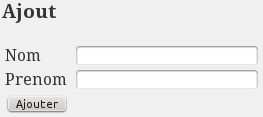
\includegraphics[]{formulaire-ajout-auteur}
  \caption{Formulaire d'ajout d'un auteur}
\end{center}
\end{figure}

Le numéro d'identification de l'auteur est automatiquement affecté de manière
à être unique : c'est un numéro incrémenté en interne à chaque ajout d'un
auteur.

Pour chaque auteur, deux actions sont proposées : leur suppression de la table
et leur édition. L'appui sur les boutons associés, situés sur chaque ligne
d'auteur, permet d'effectuer ces actions. L'appui sur le bouton "Supprimer" va
lancera l'exécution de la requête supprimant l'auteur de la table.

L'appui sur le bouton "Editer" fait apparaître un formulaire en haut de la
page ; les champs "Nom" et "Prenom" sont préremplis avec le nom de le prénom
de l'auteur édité et peuvent être modifié.

Par la suite, l'appui sur le bouton "Valider" applique les modifications mais
ne fait pas disparaître le formulaire apparu pour des raisons de convenance
mais il est néanmoins mis à jour pour rendre compte des modifications
apportées à la base.
Il est en effet pratique de pouvoir appliquer un ensemble de modifications
sans avoir à réappuyer sur le bouton "Editer" à chaque fois.
Par exemple, pour la table histoire, de nombreuses modifications différentes
peuvent être effectuées suite à l'appui sur le bouton "Editer" d'une histoire
: 
\begin{itemize}
	\item modification du titre et de l'année de parution ;
	\item ajouts d'auteurs ;
	\item suppression d'auteurs.
\end{itemize}

\begin{figure}[h!]
\begin{center}
\noindent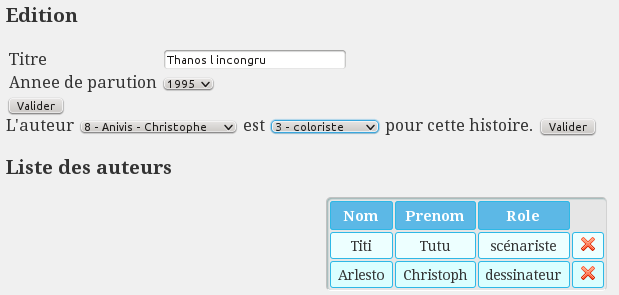
\includegraphics[]{formulaire-edition-histoire}
  \caption{Formulaire d'édition d'une histoire}
\end{center}
\end{figure}

Devoir appuyer sur éditer à chaque ajout d'un auteur, par exemple, aurait été
contraignant.

Depuis la page d'accueil il est également possible d'accéder aux pages
permettant d'effectuer les différentes requêtes. La page "Requêtes spéciales"
permet d'accéder aux requêtes de consultation et la page "Statistiques" permet
d'effectuer les requêtes de statistiques. Dans ces deux pages, le principe est
identique pour effectuer une requête : 
\begin{itemize}
	\item un menu déroulant permet de choisir la requête voulu ;
	\item l'appui sur le bouton "Valider" fait apparaître le choix des paramètres de cette
		requête ;
	\item une fois les paramètres choisis, l'appui sur le nouveau bouton
		"Valider" donne le résultat sous la forme d'une table. Si la table de
		résultat est vide alors le message "Ressource vide" est affiché.
\end{itemize}

\begin{figure}[h!]
\begin{center}
\noindent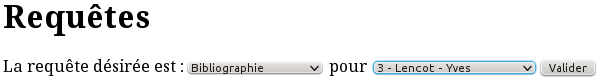
\includegraphics[]{choix-requete}
  \caption{Menu de choix des requêtes}
\end{center}
\end{figure}

\paragraph{Remarque}
Un effort a été fait pour essayer empêcher les injections SQL en formatant
les entrée de l'utilisateur. Pour cela, l'utilisation de la fonction "sprintf"
permet de forcer l'entrée de l'utilisateur à être traitée comme un nombre
lorsque cela doit être le cas. Lorsque l'utilisateur a la possibilité
d'entrer des chaînes de caractères, la fonction "mysql\_real\_escape\_string"
a été employé afin de protéger les requêtes SQL de caractères spéciaux.

\end{document}
